\documentclass[border=10pt]{standalone}

\usepackage{tikz}
\usepackage{tikzsymbols}
\usetikzlibrary{calc,patterns,shapes.geometric}

\def\centerarc[#1](#2)(#3:#4:#5){\draw[#1] ($(#2)+({#5*cos(#3)},{#5*sin(#3)})$) arc (#3:#4:#5);}

\begin{document}
	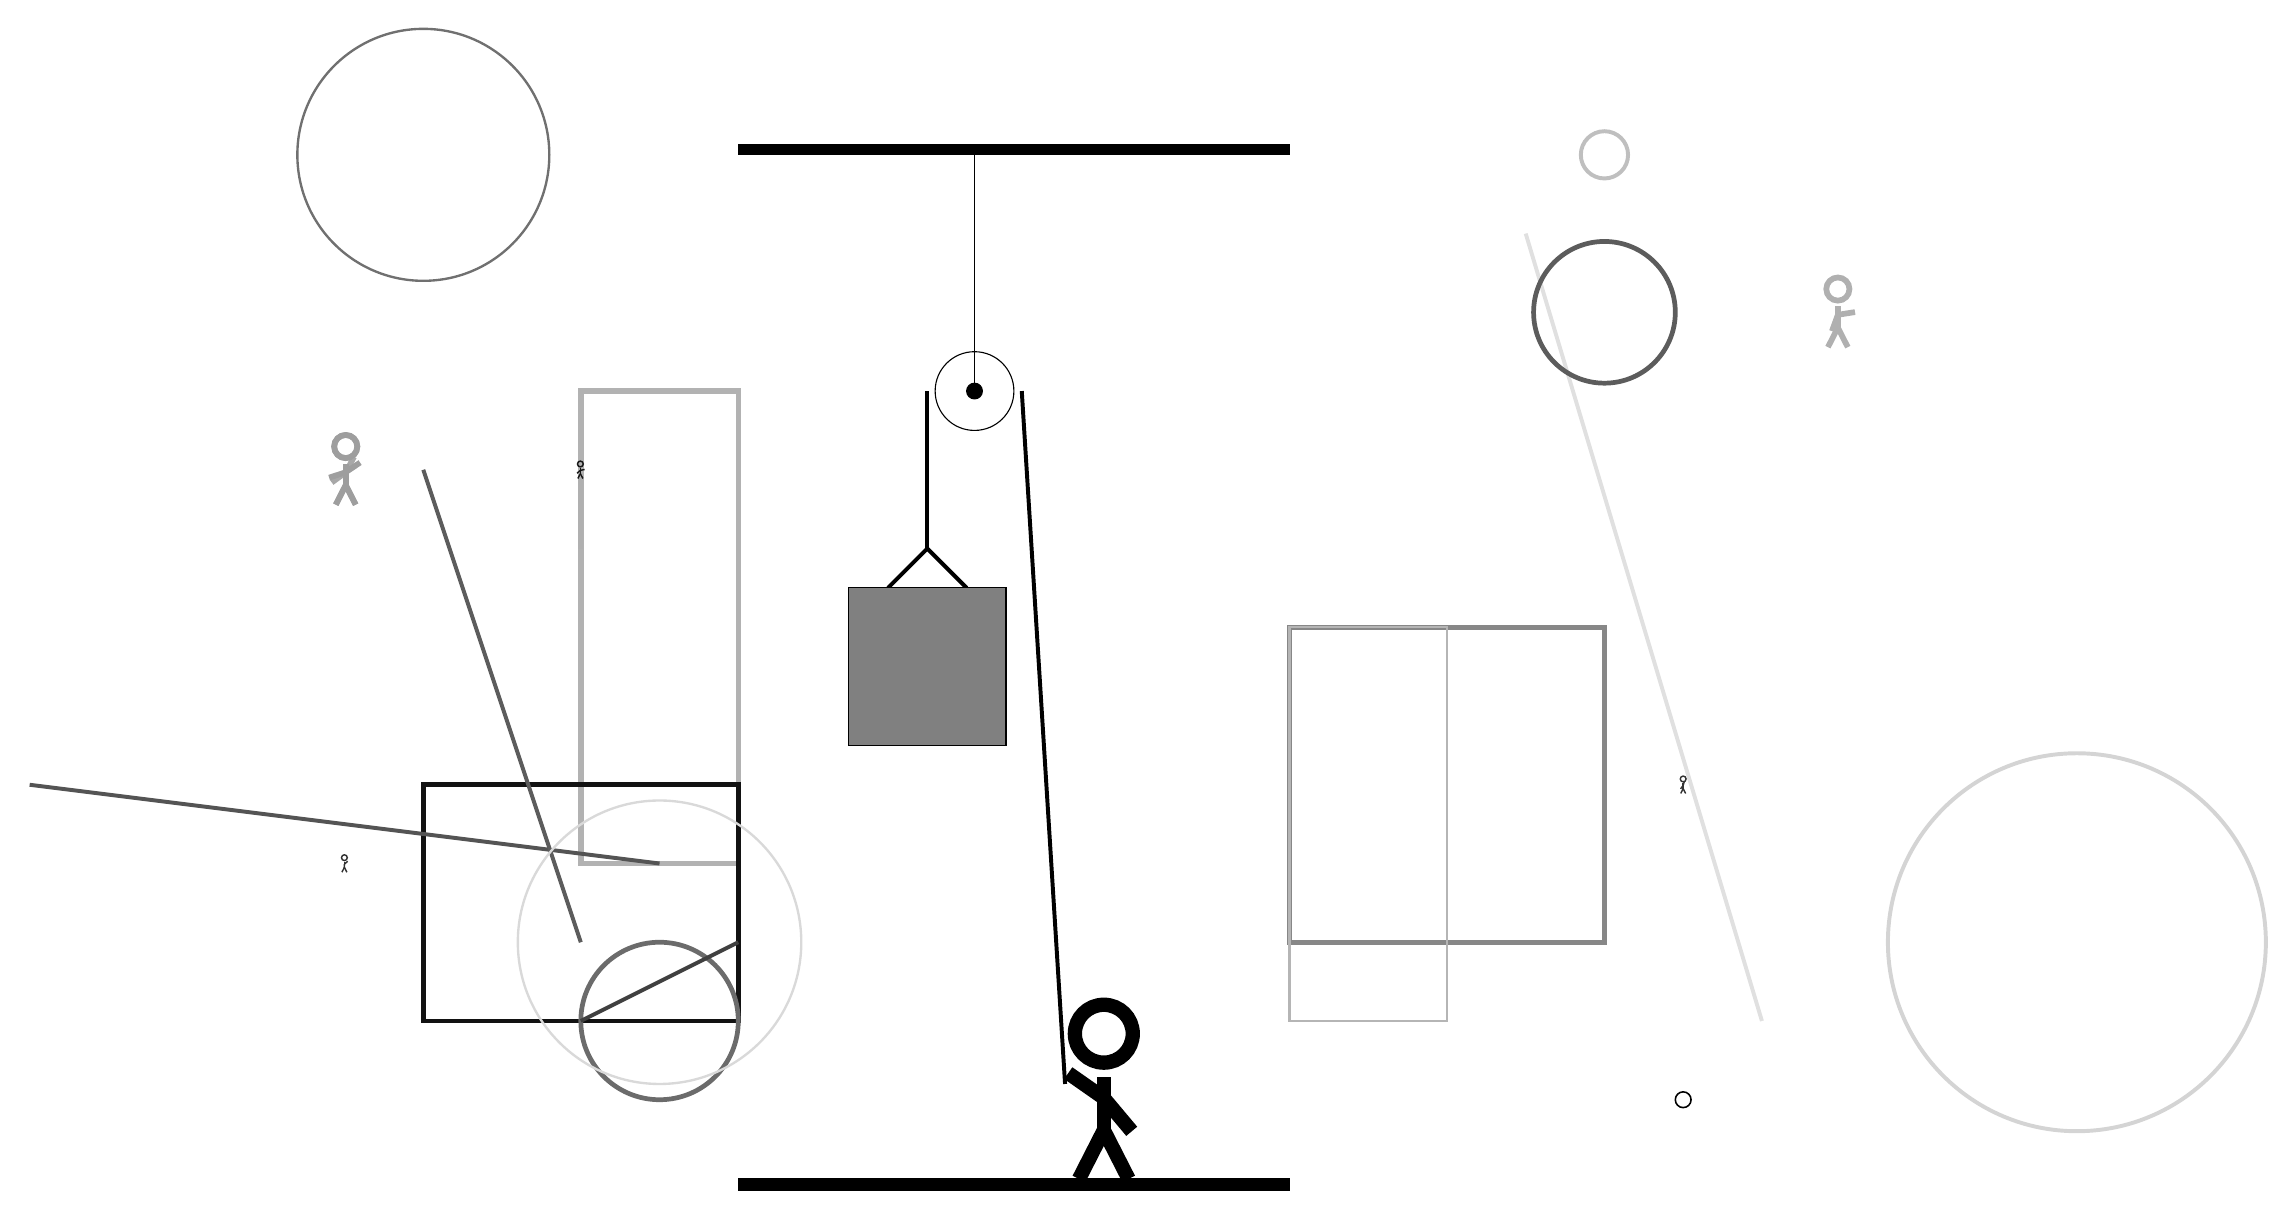
\begin{tikzpicture}
		%%%%% START %%%%%
		
		\draw[fill=black] (-2, 10) rectangle (5, 10.125);
		
		\draw (1, 7) circle (0.5);
		\draw[fill=black] (1, 7) circle (0.1);
		\draw (1, 10) -- (1, 7);
		
		\draw[line width=0.5mm] (-0.1, 4.5) -- (0.4, 5.0) -- (0.9, 4.5);
		\draw[fill=black!50] (-0.6, 4.5) rectangle (1.4, 2.5);
		
		\draw[line width=0.5mm] (0.4, 7) -- (0.4, 5.0);
		\centerarc[line width=0.5mm](1, 7)(0:180:0.6);
		\draw[line width=0.5mm](1.6, 7) -- (2.15, -1.8);
		
		\draw[line width=0.5mm, color=black!12](8, 9) -- (11, -1);
		
		\draw[line width=0.7mm, color=black!30] (-2, 7) rectangle (-4, 1);
		\draw[line width=0.6mm, color=black!93] (-2, 2) rectangle (-6, -1);
		\draw [line width=0.5mm, color=black!17](15, 0) circle (2.4);
		\draw [line width=0.5mm, color=black!25](9, 10) circle (0.3);
		\draw[line width=0.6mm, color=black!31] (-4, 5) rectangle (-4, 6);
		
		\node[line width=0.2mm, color=black!34] at (-7, 6) {\Strichmaxerl[4][36][62]};
		\draw[line width=0.5mm, color=black!67](-3, 1) -- (-11, 2);
		\draw[line width=0.6mm, color=black!47] (5, 0) rectangle (9, 4);
		
		\node[line width=0.5mm, color=black!91] at (-4, 6) {\Strichmaxerl[1][40][13]};
		
		\draw[line width=0.5mm, color=black!64](-6, 6) -- (-4, 0);
		\node[line width=0.6mm, color=black!81] at (-7, 1) {\Strichmaxerl[1][87][41]};
		\node[line width=0.7mm, color=black!31] at (12, 8) {\Strichmaxerl[4][70][9]};
		
		\draw[line width=0.3mm, color=black!29] (7, 4) rectangle (5, -1);
		\draw [line width=0.3mm, color=black!56](-6, 10) circle (1.6);
		\node[line width=0.6mm, color=black!38] at (-7, 6) {\Strichmaxerl[4][18][34]};
		
		\draw [line width=0.6mm, color=black!58](-3, -1) circle (1.0);
		\node[line width=0.3mm, color=black!80] at (10, 2) {\Strichmaxerl[1][53][74]};
		\draw [line width=0.6mm, color=black!64](9, 8) circle (0.9);
		\draw [line width=0.3mm, color=black!15](-3, 0) circle (1.8);
		\draw [line width=0.2mm, color=black!100](10, -2) circle (0.1);
		
		\draw[line width=0.5mm, color=black!75](-4, -1) -- (-2, 0);
		
		\node at (2.6, -1.9) {\Strichmaxerl[10][-35][-50]};
		
		\draw[fill=black] (-2, -3) rectangle (5, -3.15);
		
		%%%%% END %%%%%
	\end{tikzpicture}
\end{document}